
\subsection{. Explain in detail how you implemented the circuit
breaker
.}

We have created a \textit{circuit-breaker} by using Netflix Hystrix fault tolerance library. It calls the web service wit all url options mentioned in the description of part 1. For every service of serviceapi we have a fallback method. If the webservice is down then \textit{circuit-breaker} application will send the message that particular service is not working at the moment. You can see the design here in the diagram:

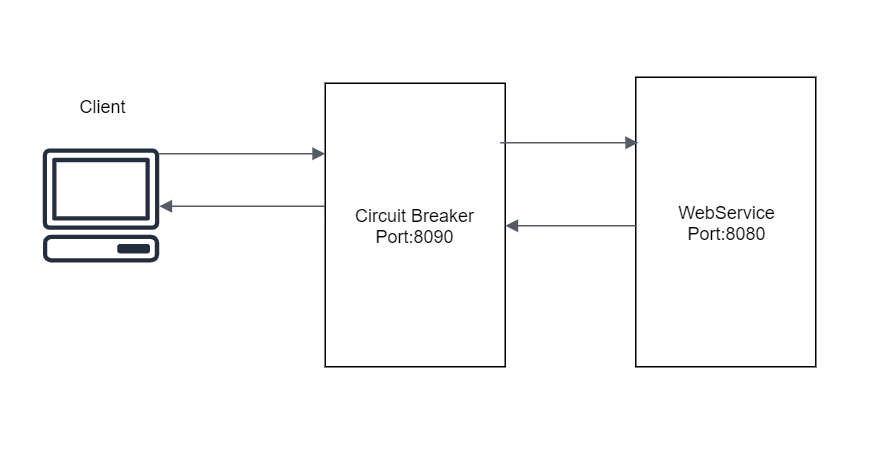
\includegraphics[keepaspectratio,width=0.8\textwidth,angle=0]{images/Circuit.PNG}
